
Linear Meld (LM) is a \emph{forward chaining} logic programming language in the
style of Datalog~\cite{Ullman:1990:PDK:533142}. The program is defined as a
\emph{database of facts} and a set of \emph{derivation rules}.  Initially, we
populate the database with the program's axioms and then determine which
derivation rules can be applied by using the current database. Once a rule is
applied, we derive new facts, which are then added to the database.  If a rule
uses linear facts, they are consumed and thus deleted from the database.  The
program stops when we reach \emph{quiescence}, that is, when we can no longer
apply any derivation rules.

LM departs from Datalog by making the database of facts a graph data structure
where each node contains a fraction of the database. Derivation rules are then
restricted so that they are only allowed to manipulate facts belonging to the
same node. This restriction allows multiple nodes of the graph to perform
independent rule derivations at the node level, thus introducing concurrency in
the program. Communication between nodes arises when a derivation rule derives a
fact that is in another node.

\section{A taste of LM}

In order to understand how LM programs are written, we now present and discuss
three basic LM programs.

\subsection{First example: key/value dictionary}

\begin{figure}[ht]
{\scriptsize
\begin{Verbatim}[numbers=right]
type left(node, node).
type right(node, node).
type linear value(node, int Key, string Value).
type linear replace(node, int Key, string Value).

replace(A, K, New),
value(A, K, Old)
   -o value(A, K, New). // we found our key

replace(A, RKey, RValue),
value(A, Key, Value),
!left(A, B),
RKey < Key
   -o value(A, Key, Value),
      replace(B, RKey, RValue). // go left

replace(A, RKey, RValue),
value(A, Key, Value),
!right(A, B),
RKey > Key
   -o value(A, Key, Value),
      replace(B, RKey, RValue). // go right

// initial configuration
!left(@0, @1).     !right(@0, @2).
!left(@1, @3).     !right(@1, @4). 
!left(@2, @5).     !right(@2, @6).

value(@0, 3, "a").   value(@1, 1, "b").
value(@2, 5, "c").   value(@3, 0, "d").
value(@4, 2, "e").   value(@5, 4, "f").
value(@6, 6, "g").

// update key 6 to value "x"
replace(@0, 6, "x").
\end{Verbatim}
}
\caption{LM program for replacing a key's value in a binary tree dictionary.}
\label{code:btree_replace}
\end{figure}

Our first example, shown in Fig.~\ref{code:btree_replace}, implements the key
update operation for a binary tree represented as a key/value dictionary. Each
LM node represents a binary tree node.  We first declare all the predicates
(lines 1-4), which represent the kinds of facts we are going to use. Note that
the first argument of every predicate must be typed as \texttt{node} because the
first argument indicates where the node lives in the graph. Predicates
\texttt{left/2} and \texttt{right/2} are persistent while \texttt{value/3} and
\texttt{replace/3} are linear. Persistent predicates are preceded with a
\texttt{!} symbol in LM rules for improved readability. Linear predicate
\texttt{value/3} assigns a key/value pair to a node that can be updated later.
The \texttt{replace/3} linear predicate represents an update operation where the
key in the second argument will be updated to the value in the third argument.

The algorithm uses three rules for the three possible cases of updating a key's
value: the first rule (lines 6-8) performs the update by removing
\texttt{replace(A, K, New)} and \texttt{value(A, K, Old)} and deriving
\texttt{value(A, K, New)}; the second rule (lines 10-15) recursively picks the
left branch for the update operation by deleting \texttt{replace(A, RKey,
RValue)} and re-deriving it at node \texttt{B}; and the third rule (lines
17-22) picks the right branch. Note that in all the rules, the body of
each rule uses facts from the same node (in this particular case,
\texttt{A}), but the head of the rule may derive facts in other
nodes (e.g., the second and third rules) because a node variable was
instantiated in the body of the rule. Moreover, persistent facts used in
the body of the rule are not deleted after rule application - only linear
facts are. The axioms of this program are presented in lines 24-35 and
they describe the initial binary tree configuration, including keys and
values.  The axiom \texttt{update(@0, 6, "x")} instantiated at the root
node \texttt{@3} manifests the intent to change the value of key 6 to 7.

Fig.~\ref{fig:btree_trace} represents the trace of the algorithm. The program
database is partitioned by the seven nodes using the first argument of each
fact. In Fig.~\ref{fig:btree_trace}~(a), we present the database filled with the
program's axioms. Next, we follow the right branch using rule 3 since $6 > 3$
(Fig.~\ref{fig:btree_trace}~(b)).  We use the same rule again in
Fig.~\ref{fig:btree_trace}~(c) where we finally reach the key 6. Here, we apply
rule 1 and \texttt{value(@6, 6, "g")} is updated to \texttt{value(@6, 6, "x")}.

\begin{figure}[h]
        \centering
        \begin{subfigure}[b]{0.5\textwidth}
                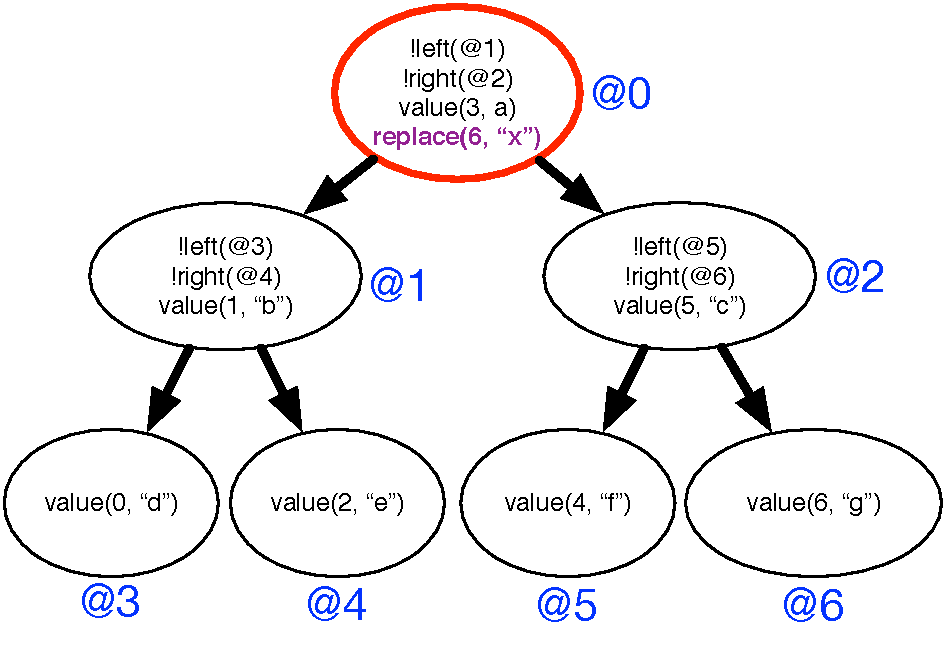
\includegraphics[width=\textwidth]{figures/btree/btree_trace1}
                \caption{Initial database. Replace axiom instantiated at the
                   \texttt{@3} root node.}
                \label{fig:btree_trace1}
        \end{subfigure}%
        ~
        \begin{subfigure}[b]{0.5\textwidth}
                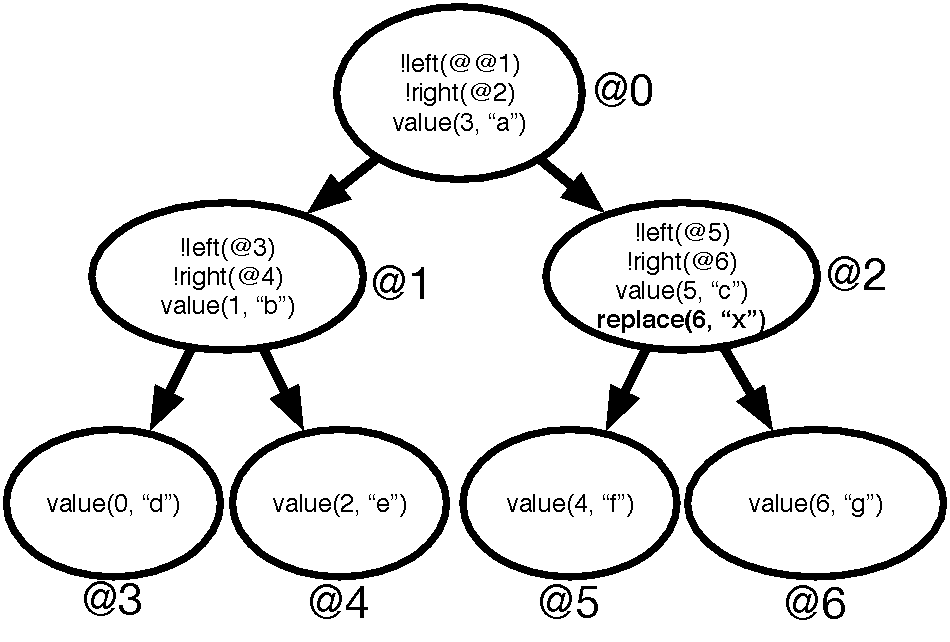
\includegraphics[width=\textwidth]{figures/btree/btree_trace2}
                \caption{After applying rule 3 at node \texttt{@3}. Replace fact
                   sent to node \texttt{@5}.}
                \label{fig:btree_trace2}
        \end{subfigure}\\
        \begin{subfigure}[b]{0.5\textwidth}
                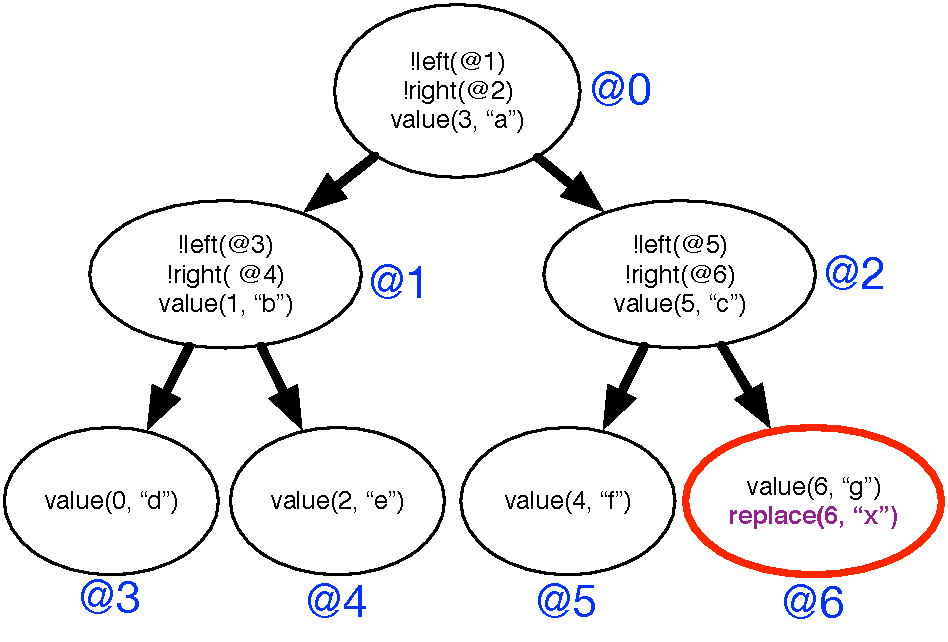
\includegraphics[width=\textwidth]{figures/btree/btree_trace3}
                \caption{After applying rule 3 at node \texttt{@5}. Replace fact
                   reaches node \texttt{@6}.}
                \label{fig:btree_trace3}
        \end{subfigure}%
        ~
        \begin{subfigure}[b]{0.5\textwidth}
                  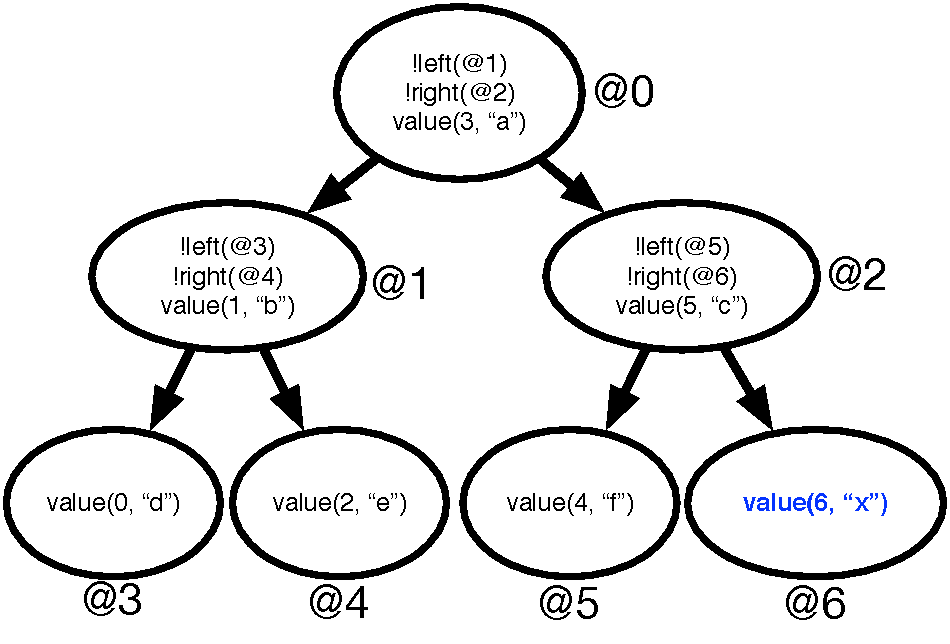
\includegraphics[width=\textwidth]{figures/btree/btree_trace4}
                  \caption{After applying rule 1 at node \texttt{@6}. Value of key 6 has changed to 7.}
                  \label{fig:btree_trace4}
          \end{subfigure}
        \caption{An execution trace for the binary tree dictionary
           algorithm. The first argument of each fact was dropped and the
           address of the node was placed beside it.}\label{fig:btree_trace}
\end{figure}

The present example offers many opportunies for concurrency. If we have multiple
\texttt{replace/3} facts on different nodes, we can perform multiple value
updates at the same time without introducing any kind of database inconsistency.

\subsection{Second example: message routing}

Fig.~\ref{code:message} shows a second LM program, a message routing program
that simulates message transmission through a network of nodes.  Predicate
\texttt{edge/2} represents the connections between nodes, predicate
\texttt{message/3} contains the message content and the route list, and
predicate \texttt{processed/2} keeps count of the number of messages routed at
each node.

\begin{figure}[h!]
\scriptsize\begin{Verbatim}[numbers=left]
type edge(node, node Neighbor).
type linear message(node, string Content, list node Routing).
type linear processed(node, int Total).

!edge(A, B),
message(A, Content, [B | L]),
processed(A, N)
   -o message(B, Content, L),
      processed(A, N + 1).

message(A, Content, []),
processed(A, N)
   -o processed(A, N + 1).

!edge(@1, @2). !edge(@2, @3). !edge(@3, @4). !edge(@1, @3).
processed(@1, 0). processed(@2, 0). processed(@3, 0). processed(@4, 0).
message(@1, "hello world", [@3, @4]).
\end{Verbatim}
\caption{Code for routing messages in a graph. There is only one message ("hello
world") to route through nodes \texttt{@3} and \texttt{@4}.}
\label{code:message}
\end{figure}

The first rule (lines 5-9) grabs the next node in the route list (third argument
of \texttt{message/3}) and ensures that a communication edge exists
(through \texttt{edge(A,B)}). We increase the number of processed messages by
consuming \texttt{processed(A,~N)} and deriving \texttt{processed(A,~N+1)}.
When the route list is empty, the message has reached its destination and thus
it is consumed (rule in lines 11-13).  Note that we only need to send one
message since there is only one \texttt{message} axiom (line 17).

In Fig.~\ref{fig:message_trace} we present an execution trace of the message
routing program.  The database is represented as a graph structure where the
edges represent the \texttt{edge/2} axioms. In Fig.~\ref{fig:message_trace}~(a)
the database is initialized with the program's axioms.  Note that the initial
\texttt{message/3} fact is instantiated at node \texttt{@1}. After applying rule 1,
we get the database represented in Fig.~\ref{fig:message_trace}~(b), where
the message has been derived at node \texttt{@3}. After applying rule 1
again, the message is then routed to node \texttt{@4}
(Fig.~\ref{fig:message_trace}~(c)) where it will be consumed
(Fig.~\ref{fig:message_trace}~(d)).

\begin{figure}[h]
        \centering
        \begin{subfigure}[b]{0.5\textwidth}
                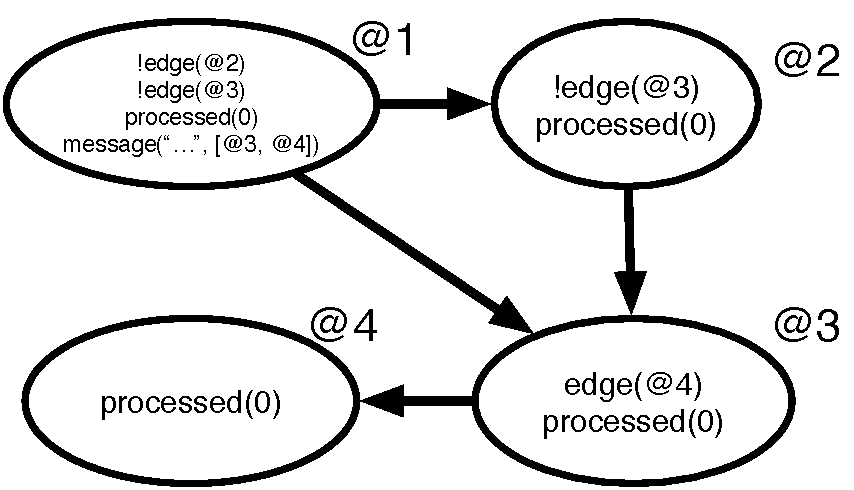
\includegraphics[width=\textwidth]{figures/message/message_trace1}
                \caption{Initial database.}
                \label{fig:message_trace1}
        \end{subfigure}%
        ~
        \begin{subfigure}[b]{0.5\textwidth}
                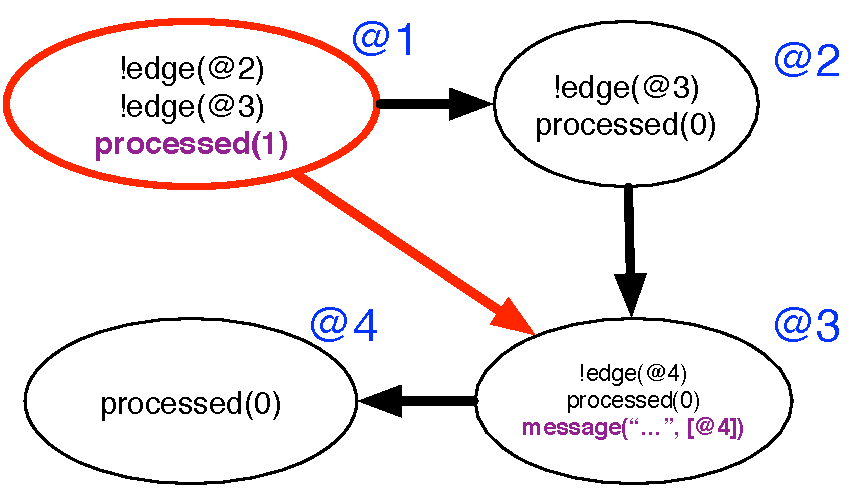
\includegraphics[width=\textwidth]{figures/message/message_trace2}
                \caption{After applying rule 1 at node \texttt{@1}.}
                \label{fig:message_trace2}
        \end{subfigure}\\
        \begin{subfigure}[b]{0.5\textwidth}
                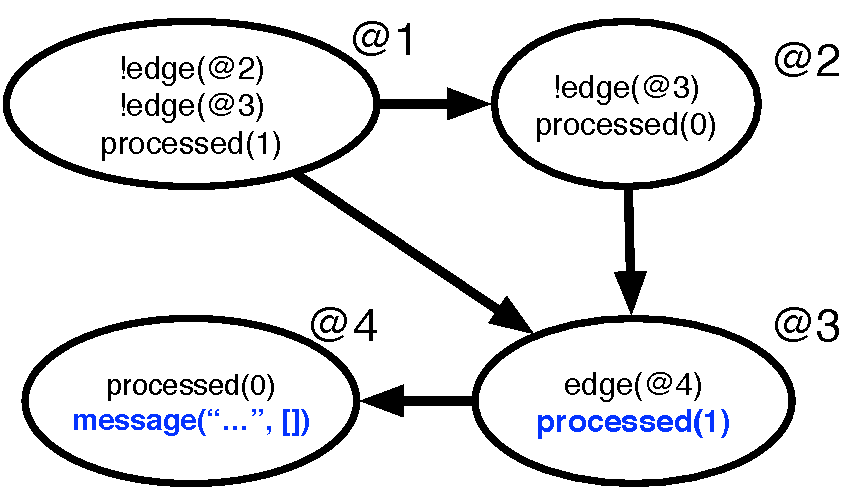
\includegraphics[width=\textwidth]{figures/message/message_trace3}
                \caption{After applying rule 1 at node \texttt{@3}.}
                \label{fig:message_trace3}
        \end{subfigure}%
        ~
        \begin{subfigure}[b]{0.5\textwidth}
                  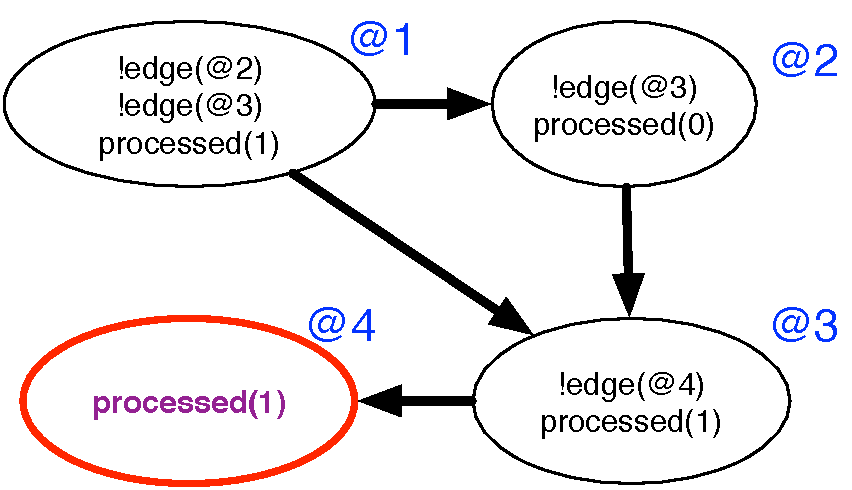
\includegraphics[width=\textwidth]{figures/message/message_trace4}
                  \caption{After applying rule 2 (nodes \texttt{@4}).}
                  \label{fig:message_trace4}
          \end{subfigure}
        \caption{An execution trace for the message program. The message "hello
        world" travels from node \texttt{@1} to node \texttt{@4}.}\label{fig:message_trace}
\end{figure}

\subsection{Third example: graph visit}

\begin{figure}[h!]
\scriptsize\begin{Verbatim}[numbers=left]
type route edge(node, node).
type linear visit(node).
type linear unvisited(node).
type linear visited(node).

// the program rules
visit(A), unvisited(A) -o
   visited(A), {B | !edge(A, B) | visit(B)}.

visit(A), visited(A) -o visited(A).

// axioms: the input data
!edge(@1, @2). !edge(@2, @3). !edge(@1, @4). !edge(@2, @4).
unvisited(@1). unvisited(@2). unvisited(@3). unvisited(@4).

visit(@1).
\end{Verbatim}
  \caption{Visit program. Nodes reachable from node \texttt{@1} will be marked
     as \texttt{visited}.}
  \label{code:visit}
\end{figure}
\normalsize

Our final example shown in Fig.~\ref{code:visit} presents another complete LM
program that, for a given graph of nodes, performs a visit to all nodes
reachable from node \texttt{@1}.  The first rule of the program (lines 7-8)
visits node \texttt{A} for the first time: fact \texttt{visited(A)} is
derived and a \emph{comprehension} construct is derived in order to go
through all the edge facts and then derive \texttt{visit(B)} for each
neighbor \texttt{B}.  The second rule (line 10) is fired when the node is
already visited more than once: we keep the \texttt{visited} fact and delete
\texttt{visit/1}.  Node \texttt{@1} starts with the \texttt{visit(@1)} fact
(line 16).

Fig.~\ref{fig:exec_trace} shows a possible execution trace for the visit
program.  After applying the first rule at node \texttt{@1} we get the database
in Fig~\ref{fig:exec_trace}~(b).  Note that node \texttt{@1} is now visited and
nodes \texttt{@2} and \texttt{@4} now have the fact \texttt{visit/1}. At this
point we could either apply rule 1 at node \texttt{@2} or at node \texttt{@4}.
For this specific trace, we apply the rule at node \texttt{@2}, resulting in
Fig.~\ref{fig:exec_trace}~(c). Node \texttt{@4} now has 2 \texttt{visit/1}
facts, thus we can apply rule 1 followed by rule 2, therefore consuming both
\texttt{visit/1} facts and deriving \texttt{visited/1}. In addition, we can also
apply rule 1 at node \texttt{@3} to reach the state of
Fig.~\ref{fig:exec_trace}~(d).

\begin{figure}[h]
        \centering
        \begin{subfigure}[b]{0.5\textwidth}
                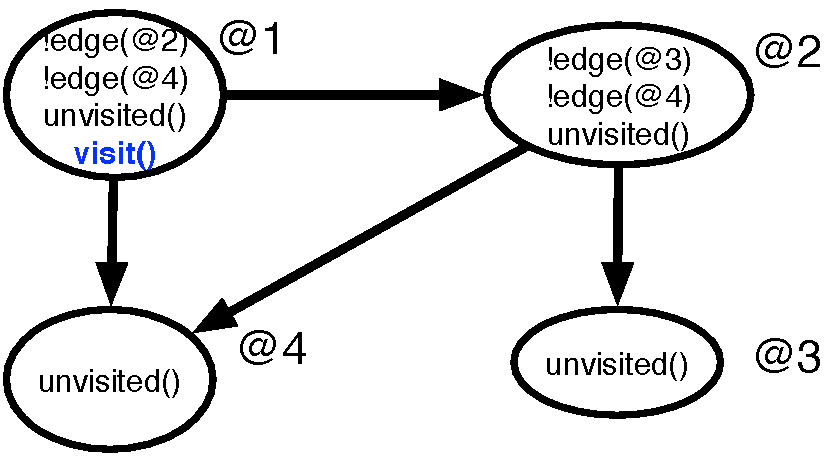
\includegraphics[width=\textwidth]{figures/visit/trace1}
                \caption{Initial database.}
                \label{fig:exec_trace1}
        \end{subfigure}%
        ~ %add desired spacing between images, e. g. ~, \quad, \qquad etc.
          %(or a blank line to force the subfigure onto a new line)
        \begin{subfigure}[b]{0.5\textwidth}
                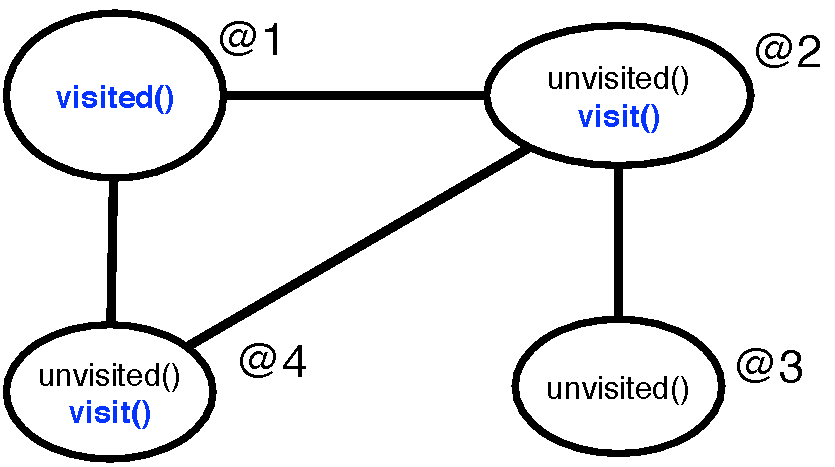
\includegraphics[width=\textwidth]{figures/visit/trace2}
                \caption{After applying rule 1 at node \texttt{@1}.}
                \label{fig:exec_trace2}
        \end{subfigure}\\
        \begin{subfigure}[b]{0.5\textwidth}
                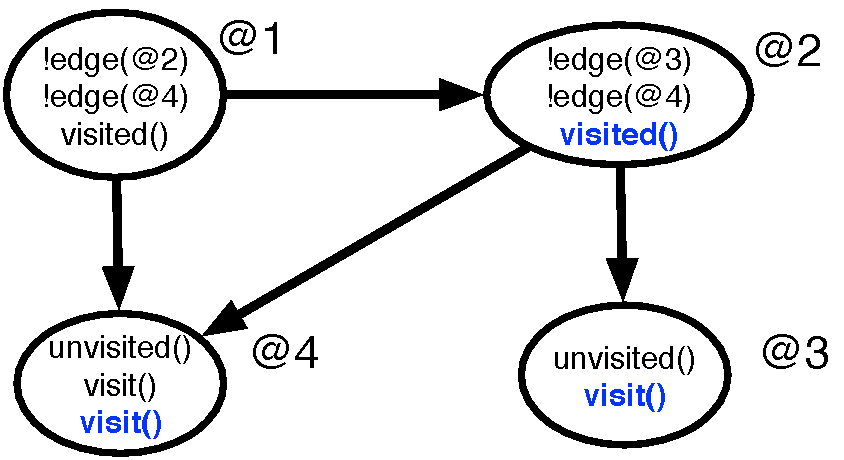
\includegraphics[width=\textwidth]{figures/visit/trace3}
                \caption{After applying rule 1 at node \texttt{@2}.}
                \label{fig:exec_trace3}
        \end{subfigure}%
        ~ %add desired spacing between images, e. g. ~, \quad, \qquad etc.
         %(or a blank line to force the subfigure onto a new line)
        \begin{subfigure}[b]{0.5\textwidth}
                  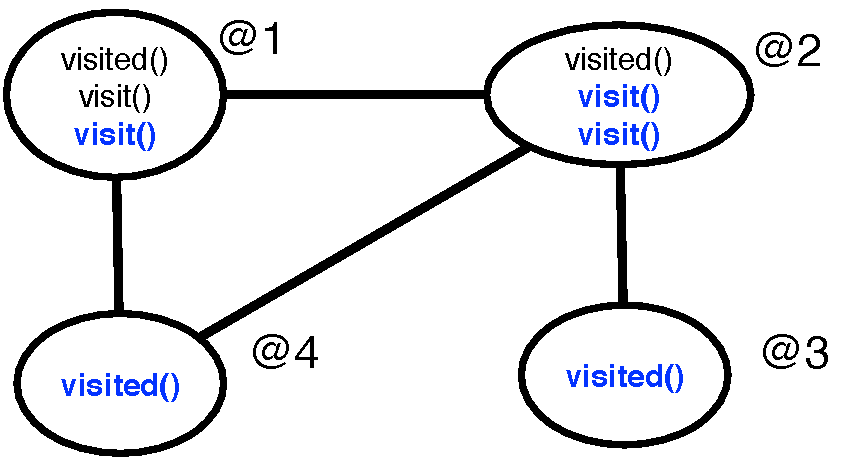
\includegraphics[width=\textwidth]{figures/visit/trace4}
                  \caption{After applying rule 1 and 2 (nodes \texttt{@3},
                        \texttt{@4}).}
                  \label{fig:exec_trace4}
          \end{subfigure}
        \caption{A possible execution trace for the visit program.}\label{fig:exec_trace}
\end{figure}

\subsubsection{Correctness of graph visit}

It is possible to prove that if a graph is connected, then all the nodes will be
become \texttt{visited}, regardless of the order in which we apply the rules.
First, we define what is a visit graph:

\begin{definition}[Visit Graph]
A visit graph is an ordered pair $G = (N, E)$ comprising a set $N$ of nodes together
with a set $E$ of edges. Set $E$ contains pairs $(A, B)$ that correspond to
facts \texttt{\bang edge(A, B)}. For every pair $(A, B) \in E$ there is also a
pair $(B, A) \in E$, representing an undirected edge.
\end{definition}

To prove the correctness property of the program, we first define the main
\emph{invariant} of the program:

\begin{invariant}[Node state]
A node is either \texttt{visited} or \texttt{unvisited}
\end{invariant}
\begin{proof}
Using the axioms we know all nodes start as \texttt{unvisited}.

Rule 1 changes a node from \texttt{unvisited} to \texttt{visited}, while rule 2
keeps the node \texttt{visited}, proving the invariant.
\end{proof}

With this invariant, it is now possible to classify nodes of the graph $G$
according to their state:

\begin{definition}[Node sets] \texttt{visited} nodes are contained in set $V$,
while \texttt{unvisited} nodes are in set $U$. From the node state invariant, we
know that $V \cup U = N$ and $V \cap U = \emptyset$.
\end{definition}

We can now prove an important lemma about sets $V$ and $U$:

\begin{invariant}[Visited set]
Visited set $V$ always increases or stays the same size. The inverse is true for
set $U$.
\end{invariant}
\begin{proof}
Initially, $V = \emptyset$ and $U = N$.

By rule 1, $V$ increases by 1 while $U$ decreases by 1. With rule 2, set
membership remains unchanged.
\end{proof}

In turn, since set membership changes from $U$ to $V$, we now prove the
following:

\begin{lemma}[Edge visits]
The program generates at most one \texttt{visit} per directed edge.
\end{lemma}
\begin{proof}
From the visited set invariant, we know that once nodes become members of set $V$,
they no longer return to set $U$, therefore rule 1 applies once per
node. This rule generates a \texttt{visit} fact per edge.
\end{proof}

In order to prove that all the nodes in the graph are visited, we need to make
sure that the graph is connected.

\begin{definition}[Connected graph]
A connected graph is a graph where every pair of nodes has a path between them.
\end{definition}

Finally, we prove that all nodes will become \texttt{visited}.

\begin{theorem}[Graph visit correctness]
If graph $G$ is connected, set $V$ will eventually include all nodes in $N$,
while $U = \emptyset$.
\end{theorem}
\begin{proof}
Proof by induction.

\begin{itemize}
   \item Base case: axiom \texttt{visit(@1)} adds node \texttt{@1} to $V$. By
   the Edge visits lemma, a \texttt{visit} fact is generate for all edges of
   \texttt{@1}.
   \item Inductive case: assume a set $V'$ and a set $U'$ that contains the
   \texttt{visited} and \texttt{unvisited} nodes, respectively. Since the graph
   is connected, there must be a node $a \in V'$ that is connected to a node $b
   \in U'$. Using the Edge visits lemma, a \texttt{visit(b)} fact is generated,
   swapping $b$ from $U'$ to $V'$.
\end{itemize}

Eventually, set $V$ will include all nodes in $N$.
\end{proof}

\section{LM Syntax}

\begin{table}[h]
\centering
\begin{tabular}{ l l c l }
  Program & $Prog$ & $::=$ & $\Sigma, D$ \\
  List Of Rules & $\Sigma$ & $::=$ & $\cdot \; | \; \Sigma, R$\\
  Database & $D$ & $::=$ & $\Gamma; \Delta$ \\
  Rule & $R$ & $::=$ & $BE \lolli HE \; | \; \forall_{x}. R \; | \; \selector{S}{y}{BE}{HE}$ \\
  Body Expression & $BE$ & $::=$ & $L \; | \; P \; | \; C \; | \; BE, BE \; | \;
\exists_{x}. BE \; | \; \one$\\
  Head Expression & $HE$ & $::=$ & $L \; | \; P \; | \; HE, HE \; | \; EE \; |
  \; CE \; | \; AE \; | \; \one$\\
  
  Linear Fact & $L$ & $::=$ & $l(\hat{x})$\\
  Persistent Fact & $P$ & $::=$ & $\bang p(\hat{x})$\\
  Constraint & $C$ & $::=$ & $c(\hat{x})$ \\
  Selector Operation & $S$ & $::=$ & $\mathtt{min} \; | \; \mathtt{max} \; | \; \mathtt{random}$\\
  
  Exists Expression & $EE$ & $::=$ & $\exists_{\widehat{x}}. SH$ \\
  Comprehension & $CE$ & $::=$ & $\comprehension{\widehat{X}}{SB}{SH}$ \\

  Aggregate & $AE$ & $::=$ & $\aggregate{A}{y}{\widehat{x}}{SB}{SH_1}{SH_2}$ \\
  Aggregate Operation & $A$ & $::=$ & $\mathtt{min} \; | \; \mathtt{max} \; | \;
\mathtt{sum} \; | \; \mathtt{count} \; | \; \mathtt{collect}$ \\
  
  Sub-Body & $SB$ & $::=$ & $L \; | \; P \; | \; SB, SB \; | \; \exists_{x}. SB$\\
  Sub-Head & $SH$ & $::=$ & $L \; | \; P \; | \; SH, SH \; | \; \one$\\
  
  Known Linear Facts & $\Delta$ & $::=$ & $\cdot \; | \; \Delta, l(\hat{t})$ \\
  Known Persistent Facts & $\Gamma$ & $::=$ & $\cdot \; | \; \Gamma, \bang p(\hat{t})$ \\
\end{tabular}
\caption{Abstract syntax of LM.}\label{tbl:ast}
\end{table}

Table~\ref{tbl:ast} shows the abstract syntax for rules in LM.  A LM program
$Prog$ consists of a list of derivation rules $\Sigma$ and a database $D$.  Each
derivation rule $R$ can be written as $BE \lolli HE$ where $BE$ is the body of a
rule and $HE$ is the head. Rules without bodies are allowed in LM and they are
called \textit{axioms} (lines 13-16 in Fig.~\ref{code:visit}). Rules without
heads are also allowed.

The body of a rule, $BE$, may contain linear ($L$) and persistent ($P$)
\emph{fact expressions} and constraints ($C$). Fact expressions are template
facts that instantiate variables (from facts in the database) such as
\texttt{visit(A)} in line 10 in Fig.~\ref{code:visit}. Variables can be used
again in the body for matching and also in the head when instantiating facts.
Constraints are boolean expressions that must be true in order for the rule
to be fired. Constraints use variables from fact expressions and are built
using a small functional language that includes mathematical operations,
boolean operations, external functions and literal values.

The head of a rule, $HE$, contains linear ($L$) and persistent ($P$) \emph{fact
templates} which are uninstantiated facts and will derive new facts. The head
can also have \emph{exists expressions} ($EE$), \emph{comprehensions} ($CE$)
and \emph{aggregates} ($AE$). All those expressions may use all the variables
instantiated in the body.

\subsubsection{Graph visit using abstract syntax}

In order to show how programs are represented using the abstract syntax
presented in Table~\ref{tbl:ast}, we present the 2 rules in the graph visit
program shown in Fig.~\ref{code:visit}:

\nopagebreak

\begin{align}
\forall_A. \mathtt{visit}(A), \; \mathtt{unvisited}(A) \lolli & \;
\mathtt{visited}(A), \; \{ B; \; \bang \mathtt{edge}(A, B); \;
\mathtt{visit}(B)\}\\
\forall_A. \mathtt{visit}(A), \; \mathtt{visited}(A) \lolli & \;
\mathtt{visited}(A)
\end{align}

Finally, axioms are represented using an empty body:

\nopagebreak

\begin{align}
\one \lolli & \bang \mathtt{edge}(@1, @2) \\
\one \lolli & \bang \mathtt{edge}(@2, @3) \\
\one \lolli & \bang \mathtt{edge}(@1, @4) \\
\one \lolli & \bang \mathtt{edge}(@2, @4) \\
\one \lolli & \bang \mathtt{unvisited}(@1)  \\
\one \lolli & \bang \mathtt{unvisited}(@2) \\
\one \lolli & \bang \mathtt{unvisited}(@3) \\
\one \lolli & \bang \mathtt{unvisited}(@4) \\
\one \lolli & \bang \mathtt{visit}(@1)
\end{align}

\subsection{Predicates and Facts}

Each fact is an association between a \emph{predicate} and a tuple of values. A
predicate is a pair with a name and a tuple of types (the argument types). LM
rules are type-checked using the predicate declarations in the header of the
program. LM has a simple type system that includes the following simples types:
\emph{node}, \emph{int}, \emph{float}, \emph{string}, \emph{bool}. Recursive
types such as \emph{list X} and \emph{pair X; Y} are also allowed.

\subsection{Selectors}

When a rule body is instantiated using facts from the database, facts are picked
non-deterministically. While our system uses an implementation dependent order
for efficiency reasons, sometimes it is important to sort facts by one of the
arguments because linearity imposes commitment during rule derivation. The
abstract syntax for this construct is $\selector{S}{y}{BE}{HE}$, where $S$ is
the selection operation and $y$ is the variable in the body $BE$ that represents
the value to be selected according to $S$. An example using concrete syntax is
as follows:

{\small
\begin{Verbatim}
[min => W | !edge(A, B), weight(A, B, W)]
                              -o picked(A, B, W).
\end{Verbatim}
}

In this case, we will order the \texttt{weight} facts by \texttt{W} in ascending
order and then try to match them. Other operations available are \texttt{max}
and \texttt{random} (to force no pre-defined order at the implementation level).

\subsection{Exists Expression}

Exist constructs ($EE$) are based on the linear logic construct of the same name
and are used to create new node addresses. We can use the new address to
instantiate new facts for the new node.  The following example illustrates the
use of the exists construct, where we derive \texttt{perform-work} at a new node
\texttt{B}.

{\small
\begin{Verbatim}
   work(A, W) -o exists B. (perform-work(B, W)).
\end{Verbatim}
}

\subsection{Comprehensions}

Sometimes we need to consume a linear fact and then immediately generate several
facts depending on the contents of the database. To solve this particular need,
we created the concept of comprehensions, which are sub-rules that are
applied with all possible combinations of facts from the database. In a
comprehension $\comprehension{\widehat{x}}{SB}{SH}$, $\widehat{x}$ is a
list of variables, $SB$ is the body of the comprehension and $SH$ is the
head.  The body $SB$ is used to generate all possible combinations for the
head $SH$, according to the facts in the database.  We have already seen
an example of comprehensions in the visit program (Fig.~\ref{code:visit}
line 8).  Here, we match \texttt{!edge(A, B)} using all the
combinations available in the database and for each combination we derive
\texttt{visit(B)}.

\subsection{Aggregates}

Another useful feature in logic programs is the ability to reduce several facts
into a single fact.  In LM we have aggregates ($AE$), a special kind of sub-rule
that works very similarly to comprehensions.  In the abstract syntax
$\aggregate{A}{y}{\widehat{x}}{SB}{SH_1}{SH_2}$, $A$ is the aggregate operation,
$\widehat{x}$ is the list of variables introduced in $BE$, $SH_1$ and $SH_2$
and $y$ is the variable in the body $SB$ that represents the values to be
aggregated using $A$. Like comprehensions, we use $\widehat{x}$ to try all
the combinations of $SB$, but, in addition to deriving $SH_1$ for each
combination, we aggregate the values represented by $y$ into a new $y$
variable that is used inside the head $SH_2$.

To better understand aggregates, let's consider a database with the following
facts and a rule:

{\small
\begin{Verbatim}
   price(@1, 3).
   price(@1, 4).
   price(@1, 5).
   count-prices(@1).
   count-prices(A) -o [sum => P | . | price(A, P) | 1 | total(A, P)].
\end{Verbatim}
}

By applying the rule, we consume \texttt{count-prices(@1)} and derive the
aggregate which consumes all the \texttt{price(@1, P)} facts.  These are summed
and \texttt{total(@1,~12)} is derived. LM provides several aggregate operations,
including the \texttt{min} (minimum value), \texttt{max} (maximum value),
\texttt{sum} (add all numbers), \texttt{count} (count combinations) and
\texttt{collect} (collect items into a list).

\section{Operational Semantics}

As said before, the first argument of every predicate must be typed as a
\emph{node}.  For distribution purposes, the body of all derivation rules can
only use facts from the same node in order to avoid concurrency issues.
However, the facts in the head may refer to other nodes, as long as those nodes
are instantiated in the body of the rule.  We drew some inspiration from the
Linda system~\cite{linda} mentioned early on, where the tuple space contains
the data and is used by the processors to communicate and do computation.  This
differs from imperative languages, since in those languages data and computation
are two separate entities.

The execution is performed at the node level and happens non-deterministically
(i.e., any node can be picked to run). This means that the programmer cannot
expect that facts coming from different nodes will be considered as a whole or
partially since the process is non-deterministic. The operational semantics
promises that rule derivations are performed atomically, therefore if a rule
sends many facts to a node then the target node will receive them all at once.
Under these restrictions, computation can then be parallelized by processing
many nodes concurrently.

Each rule in LM has a defined priority that is inferred from its position in the
source file.  Rules at the beginning of the file have higher priority. At the
node level, we consider all the new facts that have been not consider before to
create a priority queue of \emph{candidate rules}.  The queue of candidate rules
is then applied (by priority) and updated as new facts are derived or consumed.
Section~\ref{sec:core_engine} gives details in how our implementation manages
the set of candidate rules.

\section{Summary}

In this chapter we gave an overview of the LM language, including its syntax and
operational semantics.  We also explained how to write programs using all the
facilities provided by LM, including linear facts and comprehensions. We also
explained how to informally prove a graph visit program.
The implicit parallelism of LM arising from database partitioning and rule
restriction allows programs to be run in a concurrent fashion.
